% ESCAPE user manual -- English version.
% Translation of documentation/escape.pdf (Spanish original, April 2025).
%
% Build:  cd documentation && pdflatex escape_en.tex && pdflatex escape_en.tex
% (run twice so the table of contents is up to date)
\documentclass[12pt,a4paper]{book}

\usepackage[utf8]{inputenc}
\usepackage[T1]{fontenc}
\usepackage[english]{babel}
\usepackage[a4paper,margin=1in]{geometry}
\usepackage{amsmath,amssymb}
\usepackage{textcomp}
\usepackage{graphicx}
\usepackage{array}
\usepackage{booktabs}
\usepackage[table]{xcolor}
\usepackage{listings}
\usepackage{enumitem}
\usepackage{indentfirst}
\usepackage[hidelinks,
            pdftitle={ESCAPE -- User Manual},
            pdfauthor={Luis Moya, Julio Ram\'irez, Erick Mas, Shunichi Koshimura},
            pdflang={en}]{hyperref}

% ---------------------------------------------------------------------------
% Look and feel (matches the Spanish edition)
% ---------------------------------------------------------------------------
\makeatletter
% numbers of sections/subsections end with a dot: "3.3." and "3.3.1."
\renewcommand{\thesection}{\thechapter.\@arabic\c@section.}
\renewcommand{\thesubsection}{\thechapter.\@arabic\c@section.\@arabic\c@subsection.}
% the running header must not add a second dot after the section number
\renewcommand{\sectionmark}[1]{\markright{\MakeUppercase{\ifnum\c@secnumdepth>\z@\thesection\ \fi #1}}}
\makeatother

\setlength{\emergencystretch}{3em}
\renewcommand{\labelitemi}{\scriptsize$\blacksquare$}
\setlist[itemize]{itemsep=1.1ex,topsep=1.5ex,parsep=0pt}
\setlist[enumerate]{itemsep=1.1ex,topsep=1.5ex,parsep=0pt}

\definecolor{rowgray}{gray}{0.9}
\definecolor{codegray}{gray}{0.95}

\newcolumntype{L}[1]{>{\raggedright\arraybackslash}p{#1}}
\newcolumntype{C}[1]{>{\centering\arraybackslash}p{#1}}

% inline code
\newcommand{\cmd}[1]{\texttt{#1}}
\newcommand{\escape}{ESCAPE\textsuperscript{\textregistered}}

% ---------------------------------------------------------------------------
% Listings
% ---------------------------------------------------------------------------
\lstdefinestyle{control}{
  basicstyle=\ttfamily\small,
  keywordstyle=\color{red},
  morekeywords={nodesFile,linksFile,populationsFile,stopAt,endTime,deltaT,
    graphicPrintoutPeriod,computationContinued,previousComputationFile,
    stopSimulationAt,endNumberSimulation,process,meanRayleigh,
    opcionSubdivision,anchoSubdivision,cantidadSubdivisiones,
    figureTotalEvacuadosVsSimulacion,tableTotalEvacuadosVsSimulacion,
    totalEvacuadosVsSimulacionPeriod,evacuadosVsTiempoAt},
  numbers=left,
  numberstyle=\tiny,
  numbersep=5pt,
  backgroundcolor=\color{codegray},
  frame=single,
  columns=fixed,
  keepspaces=true,
  showstringspaces=false,
  breaklines=true,
  postbreak=\mbox{\space},
  aboveskip=1.2ex,
  belowskip=1.2ex,
}
\lstdefinestyle{csvfile}{
  basicstyle=\ttfamily\small,
  backgroundcolor=\color{codegray},
  frame=single,
  frameround=tttt,
  rulecolor=\color{black!75},
  framerule=1pt,
  xleftmargin=4pt,
  xrightmargin=4pt,
  framexleftmargin=4pt,
  framexrightmargin=4pt,
  framextopmargin=4pt,
  framexbottommargin=4pt,
  columns=fixed,
  keepspaces=true,
  showstringspaces=false,
  aboveskip=1.5ex,
  belowskip=1.5ex,
}
\newenvironment{csvblock}{\par\noindent\begin{minipage}{\linewidth}}{\end{minipage}\par}
\lstdefinestyle{shell}{
  basicstyle=\ttfamily\small,
  backgroundcolor=\color{codegray},
  frame=single,
  numbers=left,
  numberstyle=\tiny,
  numbersep=5pt,
  columns=fixed,
  keepspaces=true,
  showstringspaces=false,
  breaklines=true,
  postbreak=\mbox{\space},
  aboveskip=1.2ex,
  belowskip=1.2ex,
}

% ---------------------------------------------------------------------------
% Command-reference tables (Part I)
% ---------------------------------------------------------------------------
\newlength{\colA}\setlength{\colA}{2.6cm}
\newlength{\colB}\setlength{\colB}{4.0cm}
\newlength{\colC}\setlength{\colC}{6.6cm}
\newlength{\colBC}\setlength{\colBC}{\dimexpr\colB+\colC+2\tabcolsep\relax}

\newenvironment{cmdtable}[1][Detail]{%
  \begin{center}
  \small
  \renewcommand{\arraystretch}{1.12}
  \begin{tabular}{L{\colA}C{\colB}L{\colC}}
  \toprule
  \textbf{Attribute} & \textbf{Value} & \textbf{#1}\\
  \midrule
}{%
  \bottomrule
  \end{tabular}
  \end{center}
}
% #1 value, #2 detail
\newcommand{\rowType}[2]{\rowcolor{rowgray}\textbf{Type} & \cmd{#1} & #2\\}
\newcommand{\rowDefault}[2]{\textbf{Default} & \cmd{#1} & #2\\}
% default value written in plain text instead of typewriter
\newcommand{\rowDefaultText}[2]{\textbf{Default} & #1 & #2\\}
% #1 description (spans the value and detail columns)
\newcommand{\rowDescription}[1]{\rowcolor{rowgray}\textbf{Description} & \multicolumn{2}{L{\colBC}}{#1}\\}

\begin{document}

\pagenumbering{arabic}

% ---------------------------------------------------------------------------
% Title page
% ---------------------------------------------------------------------------
\begin{titlepage}
  \centering
  \vspace*{0.5cm}
  {\LARGE\bfseries ESCAPE\par}
  \vspace{0.3cm}
  {\small\bfseries Emergency System for Calculating Adaptive Pedestrian Evacuations\par}
  \vspace{1.6cm}
  {\LARGE\bfseries User Manual\par}
  \vspace{1.5cm}
  {\small By:\par}
  \vspace{1.0cm}
  {\large\bfseries Luis Moya\par}
  {\large Department of Engineering, Pontificia Universidad Católica del Perú\par
   (PUCP), Peru\par}
  \vspace{0.9cm}
  {\large\bfseries Julio Ramírez\par}
  {\large Department of Engineering, Pontificia Universidad Católica del Perú\par
   (PUCP), Peru\par}
  \vspace{0.9cm}
  {\large\bfseries Erick Mas\par}
  {\large International Research Institute of Disaster Science\par
   (IRIDeS), Tohoku University, Japan\par}
  \vspace{0.9cm}
  {\large\bfseries Shunichi Koshimura\par}
  {\large International Research Institute of Disaster Science\par
   (IRIDeS), Tohoku University, Japan\par}
  \vspace{2.2cm}
  {\large\bfseries Funded by CONCYTEC-PROCIENCIA\par
   (Contract Number PE501078853-2022)\par}
  \vfill
  {\large April 2025\par}
  \vspace{1cm}
\end{titlepage}

% blank back of the title page (numbered, as in the Spanish edition)
\setcounter{page}{2}
\thispagestyle{plain}
\mbox{}
\clearpage

\tableofcontents

% ===========================================================================
\part{References}
% ===========================================================================

\section{List of commands}

\subsection{\texttt{nodesFile}}
\begin{cmdtable}
  \rowType{String}{Data type used for this command.}
  \rowDefault{nodes.csv}{Default name of the file that contains the intersection information.}
  \rowDescription{Name of the intersections data file.}
\end{cmdtable}

\subsection{\texttt{linksFile}}
\begin{cmdtable}[Description]
  \rowType{String}{Data type used for this command.}
  \rowDefault{links.csv}{Default name of the file that contains the street information.}
  \rowDescription{Name of the streets data file.}
\end{cmdtable}

\subsection{\texttt{populationsFile}}
\begin{cmdtable}[Description]
  \rowType{String}{Data type used for this command.}
  \rowDefault{population.csv}{Default file that contains the population.}
  \rowDescription{Name of the people data file.}
\end{cmdtable}

\subsection{\texttt{startTime}}
\begin{cmdtable}[Description]
  \rowType{Integer}{Data type used for this command.}
  \rowDefault{0}{Default value used to define the start time.}
  \rowDescription{Start time of the evacuation; it must be entered in seconds.}
\end{cmdtable}

\subsection{\texttt{process}}
\begin{cmdtable}
  \rowType{String}{Data type used for this command.}
  \rowDefault{calibration}{Default value used to define the simulation process.}
  \rowcolor{rowgray}\textbf{Description} & & Indicates the simulation process.\\
  \textbf{- Calibration} & \multicolumn{2}{L{\colBC}}{In this process the code needs to train the
    \cmd{Sarsa} algorithm so that it makes its own decisions. The calibration process allows it to
    explore and experiment with decisions in order to store the learning results; this process can be
    repeated according to the desired number of simulations.}\\
  \rowcolor{rowgray}\textbf{- Trained} & \multicolumn{2}{L{\colBC}}{In this process the \cmd{Sarsa}
    algorithm uses what it has learned. It only allows the previous learning to be used and, based
    on it, to model a simulation.}\\
\end{cmdtable}

\subsection{\texttt{stopAt}}
\begin{cmdtable}
  \rowType{String}{Data type used for this command.}
  \rowDefault{endTime}{Default option used to define the final evacuation time.}
  \rowDescription{Options for determining when to stop the evacuation. Only one is implemented:
    \cmd{endTime}.}
\end{cmdtable}

\subsection{\texttt{endTime}}
\begin{cmdtable}
  \rowType{Integer}{Data type used for this command.}
  \rowDescription{Used to enter the last evacuation time up to which the simulation is to be run.}
\end{cmdtable}

\subsection{\texttt{stopSimulationAt}}
\begin{cmdtable}
  \rowType{String}{Defines the data type as a character string.}
  \rowDefault{endNumberSimulation}{The number of simulations at which to stop.}
  \rowDescription{Options for ending the simulations. Two are implemented:
    \cmd{endNumberSimulation} and \cmd{addNumberSimulation}.}
\end{cmdtable}

\subsection{\texttt{endNumberSimulation}}
\begin{cmdtable}
  \rowType{Integer}{Defines the data type as a character string.}
  \rowDescription{Number of simulations that will be run; the last iteration of the simulation is
    entered. Note that it is mandatory to set this value.}
\end{cmdtable}

\subsection{\texttt{meanRayleigh}}
\begin{cmdtable}
  \rowType{Integer}{Data type used for this command.}
  \rowDefault{420}{Default value used for the mean of the Rayleigh distribution.}
  \rowDescription{Mean of the Rayleigh distribution (the only adjustable parameter of the
    distribution). It is used to compute the scale factor needed to obtain a number from that
    distribution. The value must be entered in seconds.}
\end{cmdtable}

\subsection{\texttt{numberLinkDivision}}
\begin{cmdtable}
  \rowType{Integer}{Data type used for this command.}
  \rowDefault{10}{Default value for the subdivision of a street.}
  \rowDescription{Number of partitions applied to the streets in order to obtain a pedestrian
    count.}
\end{cmdtable}

\subsection{\texttt{exploration}}
\begin{cmdtable}
  \rowType{Integer}{Data type used for this command.}
  \rowDefaultText{close to 0.2}{Default value used for the exploration percentage at the end of
    the simulation.}
  \rowDescription{Final exploration value. As the simulations proceed, the exploration rate changes
    until it reaches the value entered.}
\end{cmdtable}

\subsection{\texttt{graphicPrintout}}
\begin{cmdtable}
  \rowType{Logical}{Data type used for this command.}
  \rowDefault{Yes}{Enabled for exporting variables.}
  \rowDescription{Used to export the position, velocity and number of evacuees variables.}
\end{cmdtable}

\subsection{\texttt{graphicPrintoutPeriod}}
\begin{cmdtable}
  \rowType{Integer}{Data type used for this command.}
  \rowDefault{1}{Default value associated with the attribute.}
  \rowDescription{Time interval at which the variables are exported, i.e.\ the export interval. It
    can be greater than 1. It must be entered in seconds.}
\end{cmdtable}

\subsection{\texttt{listingPrintoutPeriod}}
\begin{cmdtable}
  \rowType{Integer}{Data type used for this command.}
  \rowDefault{1}{Default value associated with the attribute.}
  \rowDescription{Determines how often the results are shown in the terminal. It allows the run to
    be followed at execution time.}
\end{cmdtable}

\subsection{\texttt{pedestrianCountPeriod}}
\begin{cmdtable}
  \rowType{Integer}{Data type used for this command.}
  \rowDefault{1}{Default value associated with the attribute.}
  \rowDescription{Determines how often the count of people on the streets is calculated.}
\end{cmdtable}

\subsection{\texttt{computationContinued}}
\begin{cmdtable}
  \rowType{Logical}{Data type that indicates true or false.}
  \rowDefault{No}{Default value assigned to the attribute.}
  \rowDescription{Determines whether the calculations will be independent of a previous result.}
\end{cmdtable}

\subsection{\texttt{previousComputationFile}}
\begin{cmdtable}
  \rowType{String}{Defines the data type as a character string.}
  \rowDefault{population.csv}{Name of the default file used.}
  \rowDescription{Name of the file that contains the results of a previous simulation of the same
    city. That simulation provides experienced state values for the new simulation.}
\end{cmdtable}

\subsection{\texttt{totalEvacuatedCount}}
\begin{cmdtable}
  \rowType{Logical}{Data type that indicates true or false.}
  \rowDefault{Yes}{Default value assigned to the attribute.}
  \rowDescription{Allows exporting a file with the total number of people evacuated during the
    evacuation time of the trained process.}
\end{cmdtable}

\subsection{\texttt{pythonVersion}}
\begin{cmdtable}
  \rowType{Logical}{Data type that indicates true or false.}
  \rowDefault{No}{Default value assigned to the attribute.}
  \rowDescription{Allows using learning data obtained from the Python version.}
\end{cmdtable}

% ===========================================================================
\part{User manual}
% ===========================================================================

\chapter{Introduction}

\section{Presentation of the \texorpdfstring{\escape{}}{ESCAPE} software}
The \escape{} code uses the Sarsa algorithm to solve speed--time equations in order to evaluate
escape routes when a tsunami reaches the coasts of cities.

The main results of the evacuation of each pedestrian are the following:
\begin{itemize}
  \item Evacuation time
  \item Position
  \item Velocity
\end{itemize}

\section{Main features}
The main features of the software are the following:
\begin{itemize}
  \item \textbf{Software:} Developed in C++, a low-level programming language that guarantees more
    efficient and faster performance.
  \item \textbf{Evacuations:} Facilitates the planning and execution of urban evacuations.
  \item \textbf{Evacuation time:} Makes it possible to accurately calculate the total time required
    to evacuate the inhabitants of a city.
  \item \textbf{Destination points:} Provides tools to identify and establish strategic evacuation
    points in urban areas.
\end{itemize}

\section{Contact}
If you have any questions while using the software, you can contact us by sending an email to
receive technical assistance.

\medskip
\noindent Email addresses:\\
lmoya@pucp.edu.pe\\
julio.ramirez@pucp.edu.pe

\section{Requirements}
\begin{itemize}
  \item Language: C++ (C++17 support is required)
  \item Compiler: GCC 9.4 or higher / Clang 10.0 or higher
  \item Build tools:
    \begin{itemize}
      \item GNU Make 4.2.1 (Makefile)
      \item Operating system: Ubuntu 20.04.6 LTS or macOS
    \end{itemize}
\end{itemize}

% ---------------------------------------------------------------------------
\chapter{Fundamentals}

The Sarsa algorithm (State--Action--Reward--State--Action) was proposed by Rummery and Niranjan
under the name ``Modified Connectionist Q-Learning'' (MCQ-L). It was Rich Sutton who gave it the
name Sarsa.

The name Sarsa comes from the following chain: the main function for updating the Q value depends
on the current state of the agent ``$S_1$'', the action chosen by the agent ``$A_1$'', the reward
``$R_2$'' that the agent obtains for choosing this action, the state ``$S_2$'' that the agent enters
after performing that action, and, finally, the next action ``$A_2$'' that the agent chooses in its
new state. The result is the acronym of the quintuple $(S_t, A_t, R_{t+1}, S_{t+1}, A_{t+1})$.

\section{Sarsa algorithm}
The Sarsa algorithm is the following:
\begin{equation}
  Q_{\mathrm{new}}(S_t, A_t) \longleftarrow (1-\alpha)\,Q(S_t, A_t)
    + \alpha\left[R_{t+1} + \gamma\, Q(S_{t+1}, A_{t+1})\right]
\end{equation}
A Sarsa agent is known as a learning algorithm because it interacts with the environment and
updates the policy based on the actions taken. The Q value of a state--action pair is updated
through an error and is adjusted with a learning rate ``$\alpha$''.

The Q values represent the possible reward received at the next time step for taking action $a$ in
state $s$, plus the discounted future reward received from the next state--action observation.

An advantage of Sarsa is that it learns by itself the Q values associated with adopting the policy
it follows.

\section{Sarsa parameters}
The parameters used with Sarsa are shown below:
\begin{itemize}
  \item \texttt{Learning rate} ($\alpha$): Determines to what extent newly acquired information
    overrides old information. A factor of 0 makes the agent learn nothing, while a factor of 1
    makes the agent consider only the most recent information.
  \item \texttt{Discount factor} ($\gamma$): Determines the importance of future rewards. A discount
    factor of 0 makes the agent opportunistic or myopic, considering only current rewards. On the
    other hand, a factor close to 1 encourages the agent to seek high long-term rewards. If the
    discount factor is equal to or greater than 1, the Q value may diverge.
  \item \texttt{Initial conditions} ($Q(S_0, A_0)$): Since Sarsa is an iterative algorithm, it
    assumes an initial condition before the first update. A high or infinite initial value, also
    known as ``optimistic initial conditions'', can encourage exploration. The initial update rule
    assigns high values to all actions, increasing their probability of being chosen. The first time
    an action is taken, the reward ``$r$'' resets the initial conditions and is used to set the
    value of $Q$, allowing immediate learning in the case of deterministic rewards.
\end{itemize}

% ---------------------------------------------------------------------------
\chapter{Program structure and algorithm}

\section{Program structure}
The \escape{} software runs according to the structure shown in the following figure. It shows the
input information that the program needs, such as the streets (link), the intersections of the
streets (node) and the people (pedestrian), each with its identifier. Once all the information has
been entered, the data are processed, which consists of.

After the data have been processed, the outputs are tables and/or figures showing the number of
evacuees vs.\ time, the number of evacuees vs.\ evacuation points, and the total number of
evacuees vs.\ simulation number.

\section{List of classes}
\begin{table}[htbp]
  \centering
  \begin{tabular}{@{}ll@{}}
    \toprule
    File & Description\\
    \midrule
    \texttt{io}          & File input and output.\\
    \texttt{directory}   & Command dictionary.\\
    \texttt{node}        & Definition of intersections in a city.\\
    \texttt{link}        & Definition of streets in a city.\\
    \texttt{sublink}     & Definition of a subsection of a street.\\
    \texttt{pedestrian}  & Definition of pedestrians.\\
    \texttt{stateMatrix} & State matrix structure.\\
    \texttt{sarsa}       & Computation of the \texttt{Sarsa} algorithm.\\
    \bottomrule
  \end{tabular}
  \caption{Names of the classes used and implemented in the model.}
\end{table}

\section{Software modules}

\subsection{Node module (Intersections)}
The Node module has the following members:
\begin{itemize}
  \item \texttt{idNode}: Unique identifiers of each intersection.
  \item \texttt{coordenada}: Contains the location vector of the intersection.
  \item \texttt{linkConnectionsPtr}: A vector of the interconnected streets.
  \item \texttt{stateMatrixsExperimentadosPtr}: A vector of the experienced states.
\end{itemize}
The members \texttt{idNode} and \texttt{coordenada} are identified with the intersections file;
whereas \texttt{linkConnectionsPtr} and \texttt{stateMatrixsExperimentadosPtr} are members that are
obtained as the software processes the data.

\subsubsection*{Assignment of intersection values}
To enter the intersection values, a csv file is needed that contains the street identification
values, the position in x and the position in y.

The control file \texttt{controlDict} has the command \texttt{nodesFile} to specify the name of the
file; by default this is \texttt{node.csv}.

An example of changing the name of the intersections file is shown below:
\begin{lstlisting}[style=control]
nodesFile: intersectionsLima.csv
\end{lstlisting}

\subsection{Link module (Streets)}
The Link module has the following members:
\begin{itemize}
  \item \texttt{idLink}: Unique identifier of a street.
  \item \texttt{node1Ptr}: Pointer to the first intersection of the street.
  \item \texttt{node2Ptr}: Pointer to the second intersection of the same street.
  \item \texttt{length}: Length of the street.
  \item \texttt{width}: Width of the street.
  \item \texttt{orientacionLink}: Orientation of the street.
  \item \texttt{anchoSubdivision}: Width of each subdivision of the street.
  \item \texttt{cantidadSubdivisiones}: Number of subdivisions of the street, used for the density
    calculation.
  \item \texttt{densityLevel}: Density of the street, calculated as the maximum density among its
    subdivisions.
  \item \texttt{subdivisiones}: Vector of the \texttt{subLink} class, which represents the divisions
    of the street.
\end{itemize}

\subsubsection*{Assignment of street values}
To enter the street values, a file is needed in which the following are given: an identifier number
for the street, the two start and end points of the street, and the length and width of the street.
The control file \texttt{controlDict} has the command \texttt{linksFile} to specify the name of the
file, which by default is \texttt{link.csv}.

An example of changing the name of the streets file is shown below:
\begin{lstlisting}[style=control]
linksFile: streetsLima.csv
\end{lstlisting}

\subsubsection*{Options for subdividing a street}
There are two options for subdividing a street:
\begin{enumerate}
  \item \texttt{anchoSubdivision}
  \item \texttt{cantidadSubdivisiones}
\end{enumerate}
By default the \texttt{anchoSubdivision} option is enabled. This option divides the street
according to a fixed length for each subdivision, and from it the number of subdivisions is
calculated. If the number of subdivisions is not an integer, it is rounded and a new width is
calculated again, which is very close to the previous one; this is done because the number of
subdivisions cannot be a decimal value.

On the other hand, the second option allows entering a number of divisions for the street, from
which a single width for each subdivision will be calculated.

An example of the first option, which appears by default, for the subdivision of a street is shown
below:
\begin{lstlisting}[style=control]
opcionSubdivision: anchoSubdivision
\end{lstlisting}

\subsubsection*{Subdivision width}
To use this option it is not mandatory to choose \texttt{anchoSubdivision} in the
\texttt{opcionSubdivision} command, because that option is already the default.

It allows setting the value of the length of the subdivisions. The values can be integers or
decimals, but not fractions.

An example for the subdivision of a street is shown below:
\begin{lstlisting}[style=control]
anchoSubdivision: 12.5
\end{lstlisting}

\subsubsection*{Number of subdivisions}
To use this option it is necessary to choose \texttt{cantidadSubdivisiones} in the
\texttt{opcionSubdivision} command.

The \texttt{cantidadSubdivisiones} command allows dividing the street into an integer number of
subdivisions.

An example of using the command is shown below:
\begin{lstlisting}[style=control]
cantidadSubdivisiones: 20
\end{lstlisting}

\subsection{nodeDestino module (Evacuation points)}
The nodeDestino module has the following members:
\begin{itemize}
  \item \texttt{maxPersonasEvacuadas}: The number of people who can evacuate at this site. By
    default, this option is disabled, so each evacuation point has infinite capacity. To enable
    this option and limit the capacity, the intersections file must be modified by entering the
    value 2, followed by the maximum number of evacuees for that point.
\end{itemize}

\subsubsection*{Printing the Evacuees vs.\ Time figure for different simulations}
It shows a line with the information on the total number of people evacuated over the whole
evacuation time for certain simulations. The desired simulation number is added with the command
\texttt{totalEvacuadosVsSimulacionAt}, showing how the learning of the algorithm evolves. This
information is exported in png format.

An example of enabling the figure is shown below:
\begin{lstlisting}[style=control]
figureTotalEvacuadosVsTiempo: yes
\end{lstlisting}

\subsubsection*{Printing the Evacuees vs.\ Time table for different simulations}
It prints a table with the values of the total number of evacuees over the whole evacuation time
for certain simulations. The desired simulation number is added with the command
\texttt{totalEvacuadosVsSimulacionAt}, showing how the learning of the algorithm evolves. This
information is exported in csv format.

An example of enabling the table is shown below:
\begin{lstlisting}[style=control]
tableTotalEvacuadosVsTiempo: yes
\end{lstlisting}

\subsubsection*{Evacuation vs.\ Time for specific simulations}
The printing of the table and the figure of the total number of evacuees vs.\ time uses simulation
numbers 1, 2 and 3 by default. To change these values, the command
\texttt{totalEvacuadosVsTiempoAt} can be used, to which integer values separated by commas must be
assigned.

An example of assigning simulations is shown below:
\begin{lstlisting}[style=control]
  evacuadosVsTiempoAt 1, 5, 8;
\end{lstlisting}

\subsubsection*{Printing the Total evacuees vs.\ Simulation figure}
It shows a single-line plot with the information on the total number of people evacuated over the
course of the simulations, showing how the learning of the algorithm evolves. This information is
exported in png format.

An example of enabling the figure is shown below:
\begin{lstlisting}[style=control]
figureTotalEvacuadosVsSimulacion: yes
\end{lstlisting}

\subsubsection*{Printing the Total evacuees vs.\ Simulation table}
It shows a table with the values of the total number of evacuees over the course of the
simulations, showing how the learning of the algorithm evolves. This information is exported in
csv format.

An example of enabling the table is shown below:
\begin{lstlisting}[style=control]
  tableTotalEvacuadosVsSimulacion: yes
\end{lstlisting}

\subsubsection*{Simulation period of the Total evacuees vs.\ Simulation output}
The printing of the table and the figure of the total number of evacuees vs.\ simulation is done
every simulation, which is a default value. To change this value, the command
\texttt{totalEvacuadosVsSimulacionPeriod} can be used, to which the value of how often simulation
values are wanted must be assigned.

An example of assigning the simulation period is shown below:
\begin{lstlisting}[style=control]
  totalEvacuadosVsSimulacionPeriod 5;
\end{lstlisting}

\subsection{Time module}
The Time module has the following members:
\begin{itemize}
  \item \texttt{valorTiempo}: Value of the simulated time, which increases according to
    \texttt{deltaT}.
  \item \texttt{deltaT}: Time step value. By default, it is 1 second.
  \item \texttt{startNumberSimulation}: Value of the initial simulation. By default, it is 0.
  \item \texttt{endNumberSimulation}: Value of the last simulation. It must be entered in the
    \texttt{control.l} file.
  \item \texttt{graphicPrintoutPeriod}: Value that indicates how often the position, velocity and
    number of evacuated people variables should be exported.
  \item \texttt{pedestrianCountPeriod}: Value that indicates how often the density should be
    calculated.
\end{itemize}

\subsubsection*{Evacuation time}
This value is used to set, as a mandatory entry, the evacuation time in seconds.

An example is shown below:
\begin{lstlisting}[style=control]
endTime 800;
\end{lstlisting}

\subsubsection*{Setting the number of simulations}
This value is used to set, as a mandatory entry, the number of simulations. That is, each
simulation carries out one evacuation. Only integer values greater than 0 are accepted.

An example is shown below:
\begin{lstlisting}[style=control]
endNumberSimulation 7000;
\end{lstlisting}

\subsubsection*{Variable printing period}
This command makes it possible to print the variables at regular intervals, which are given in
seconds. For example, if the command has the value 5 and the command \texttt{endTime} is 50, then
the variables will be printed in the \texttt{data} folder at the following times: 0, 5, 10, 15, 20,
25, 30, 35, 40, 45, 50 by default.

An example is shown below:
\begin{lstlisting}[style=control]
graphicPrintoutPeriod 5;
\end{lstlisting}

\subsubsection*{Density calculation period}
This command makes it possible to count the people in each subdivision of the street in order to
then calculate the density of each subdivision and obtain the maximum value, which is assigned to
the street as its density level. For example, if the command has the value 6 and the command
\texttt{endTime} is 50, then the density will be calculated at times 0, 6, 18, 24, 30, 36, 42 and
48.

An example is shown below:
\begin{lstlisting}[style=control]
pedestrianCountPeriod 6;
\end{lstlisting}

% ---------------------------------------------------------------------------
\chapter{Installation}

This guide details the installation, simulation and post-processing process for some application
cases of the Sarsa code. The \texttt{run} directory contains demonstration cases of the use of the
algorithm and its utilities in different scenarios. Before trying to run the tutorials, the user
must make sure that Sarsa is correctly installed.

\section{Cloning the repository}
To clone the repository, run the following:
\begin{lstlisting}[style=shell]
> git clone https://github.com/juliocesar-ramirez/cplus-version.git
\end{lstlisting}

\section{Loading the variables}
The Sarsa environment variables are defined in the files of the Sarsa \texttt{/etc} directory.
\begin{lstlisting}[style=shell]
> cd cplus-version
> source bashrc
\end{lstlisting}

\section{Compiling Sarsa}
With the environment loaded, compilation of Sarsa starts by running the script in the makefile.
\begin{lstlisting}[style=shell]
> make
\end{lstlisting}

\section{Updating the code}
The source code is updated regularly. Therefore, these modifications and new files can be
downloaded using git.
\begin{lstlisting}[style=shell]
> git pull
\end{lstlisting}

% ---------------------------------------------------------------------------
\chapter{Evacuation simulation}

\section{Specification of the initial conditions}
There are two initial conditions for starting the evacuation simulation:
\begin{itemize}
  \item \textbf{Positions of the people at the start of the evacuation:} The positions where the
    people are located cannot be modified through the nodes file.
  \item \textbf{Departure time of the people at the start of the evacuation:} The time at which the
    people will begin to evacuate is an initial condition based on the Rayleigh distribution, whose
    parameter can be adjusted by the user.
\end{itemize}

\section{Inputs and outputs}
A list of files is used by the \escape{} program; some of them are inputs and others are outputs.
Likewise, some of them are optional. The input files are the following:
\begin{itemize}
  \item The streets file (mandatory) contains the list of streets of the city and their location.
  \item The intersections file (mandatory) contains information about the intersections of the
    streets.
  \item The people file (mandatory) contains information about the pedestrians and their starting
    position.
\end{itemize}

\subsection{Intersections file}
The user can change the name of the file by modifying the \texttt{nodesFile} command. The file
contains the following:
\begin{itemize}
  \item Id of the intersection, a unique number that cannot be equal to that of another
    intersection.
  \item x coordinate
  \item y coordinate
\end{itemize}
\begin{csvblock}
\begin{lstlisting}[style=csvfile]
# Example of the nodes.csv file
# id x y
0,0,0,0,1
1,20,0,0,1
2,40,0,0,1
3,60,0,0,1
4,80,0,0,1
\end{lstlisting}
\end{csvblock}
The order is not important. Lines that begin with \# are taken as comments. The number of points is
free and does not necessarily have to be the same as in the example.

\subsection{Streets file}
The user can change the name of the file by modifying the \texttt{linksFile} command. The file
contains the following:
\begin{itemize}
  \item Id of the street, a unique number that cannot be equal to that of another street.
  \item Id of the start intersection.
  \item Id of the exit intersection.
\end{itemize}
\begin{csvblock}
\begin{lstlisting}[style=csvfile]
# Example of the nodes.csv file
# id,node1,node2,width,
0,0,1,20,3
1,1,2,20,3
2,2,3,20,3
3,3,4,20,3
4,4,5,20,3
\end{lstlisting}
\end{csvblock}
The order is not important. Lines that begin with \# are taken as comments. The number of streets
is free and does not necessarily have to be the same as in the example.

\subsection{People file}
The user can change the name of the file by modifying the \texttt{populationsFile} command. The file
contains the following:
\begin{itemize}
  \item Age of the person
  \item Gender of the person, 1 if male.
  \item Category HHType
  \item Category HHID
  \item Starting intersection of the person.
\end{itemize}
\begin{csvblock}
\begin{lstlisting}[style=csvfile]
# Example of the population.csv file
# age,gender,HHType,HHID,closeNode
18,1,0,0,26
18,1,0,0,22
18,1,0,0,20
18,1,0,0,6
\end{lstlisting}
\end{csvblock}
The order is not important. Lines that begin with \# are taken as comments. The number of people is
free and does not necessarily have to be the same as in the example.

\subsection{Control file}
The user must see this file, called \texttt{controlDict}, located in the \texttt{system} directory.
Import of mandatory and optional input data, time control, export.

The file represents a control panel of the \escape{} code. It contains a number of commands whose
values can be assigned or used with their default values. All the commands are defined in the
reference manual.
\begin{lstlisting}[style=control]
nodesFile           nodes.csv;

linksFile           links.csv;

populationsFile  population.csv;

stopAt          endTime;

endTime         800;

deltaT          1;

graphicPrintoutPeriod 1;

listingPrintoutPeriod 1;

computationContinued    no;

previousComputationFile sim_000006000.csv;

# stopSimulationAt          endNumberSimulation;

# endNumberSimulation 6003;

readPedestrianMassState no;

stopSimulationAt          addNumberSimulation;
\end{lstlisting}
Lines that begin with \# are taken as comments.

\section{Starting the program}
The calculations are launched from the terminal using the command \texttt{sarsa}. The command
triggers the execution of a main script containing all the modules, functions and variables of the
code. The syntax of the command is the following:

The program is invoked by typing the command Sarsa in the terminal. The command runs a binary file
stored in the \texttt{bin} folder, which is a binary of all the scripts in the \texttt{src} folder.

The syntax of the command is the following:\nopagebreak
\begin{lstlisting}[style=shell]
> sarsa
\end{lstlisting}

\section{Example cases}
\escape{} includes three tutorial cases to show the functionalities of the code. These are available
in the \texttt{tutorials} folder.

\subsection{Grid case}
This tutorial will describe how to pre-process and post-process a case with an ideal city in the
shape of a rectangle. The geometry is shown in the figure, where the lines are the streets. The
people are initially positioned at the intersection points of the streets. The initial movement
speed of the people will be 1 m/s.

This example will show the most optimal evacuation route when the people leave from the same
starting point to their evacuation point. The configuration of the city has streets with a
characteristic pattern, which are junctions of 4 streets that form a rectangle, with a total of 25
blocks of the same shape, as shown in the following image.

Likewise, a street has a length of 20 meters and a width of 3 meters. This configuration has a
single evacuation point located at position (100, 100).

The user must enter certain information in the \texttt{controlDict}:
\begin{itemize}
  \item \texttt{endTime}: Final evacuation time with the \texttt{endTime} command.
  \item {\sloppy\texttt{endNumberSimulation}: The final number of simulations with the
    \texttt{endNumberSimulation} command.\par}
  \item \texttt{process}: Type of process with the \texttt{process} command.
  \item \texttt{meanRayleigh}: The mean value for the Rayleigh distribution.
  \item \texttt{populationsFile}: The name of the population file.
\end{itemize}
The input data about time control, reading, printing and solution values will be read from the
\texttt{controlDict} file. The user must modify it beforehand.

For the present case, the following image shows the aforementioned file, as well as the values of
the mandatory commands.

\begin{figure}[htbp]
  \centering
  
\includegraphics[width=0.85\textwidth]{figures/grid-city.png}
  \caption{Plan view of the city of the grid case.}
\end{figure}

\begin{lstlisting}[style=control]
populationsFile  populationAtPoint.csv;

process calibration;

endTime         1800;

meanRayleigh   420;

endNumberSimulation 1000;
\end{lstlisting}

There are commands whose value does not need to be specified, because their default value will be
used, which is listed in the commands section.

Once the \texttt{controlDict} has been defined, it is recommended to clean the working folder; for
this there is an external script named \texttt{Allclean}.

The program is run with the command \texttt{sarsa}. For the present case, the following image shows
the aforementioned file, as well as the values of the mandatory commands.
\begin{lstlisting}[style=shell]
***** Simu : 410 *****
epsilon greedy - exploration : 0.379363
survived pedestrian : 6195
Duration : 0 min / 3 s / 3018 ms

***** Simu : 411 *****
epsilon greedy - exploration : 0.378788
survived pedestrian : 6216
Duration : 0 min / 3 s / 3040 ms

***** Simu : 412 *****
epsilon greedy - exploration : 0.378215
survived pedestrian : 6225
Duration : 0 min / 2 s / 2899 ms

***** Simu : 413 *****
epsilon greedy - exploration : 0.377644
survived pedestrian : 6231
Duration : 0 min / 2 s / 2972 ms

***** Simu : 414 *****
epsilon greedy - exploration : 0.377074
survived pedestrian : 6220
Duration : 0 min / 3 s / 3005 ms
\end{lstlisting}

Upon completion, the results of each variable, tables with information on the number of evacuees
and validation images can be obtained.

Finally, the export of the variables allows the user to post-process the information in any other
program. The post-processing of the information with the Python language is shown below.

\subsection{Camaná case}
This example will show the evacuation of people in the district of Camaná with several evacuation
point options, all far from the beach, as shown in the following figure. The configuration is an
idealization based on the street layout of the district of Camaná, with a maximum street length of
600 meters and a width of 3 meters.

The configuration of this case is the following:

\begin{figure}[htbp]
  \centering
  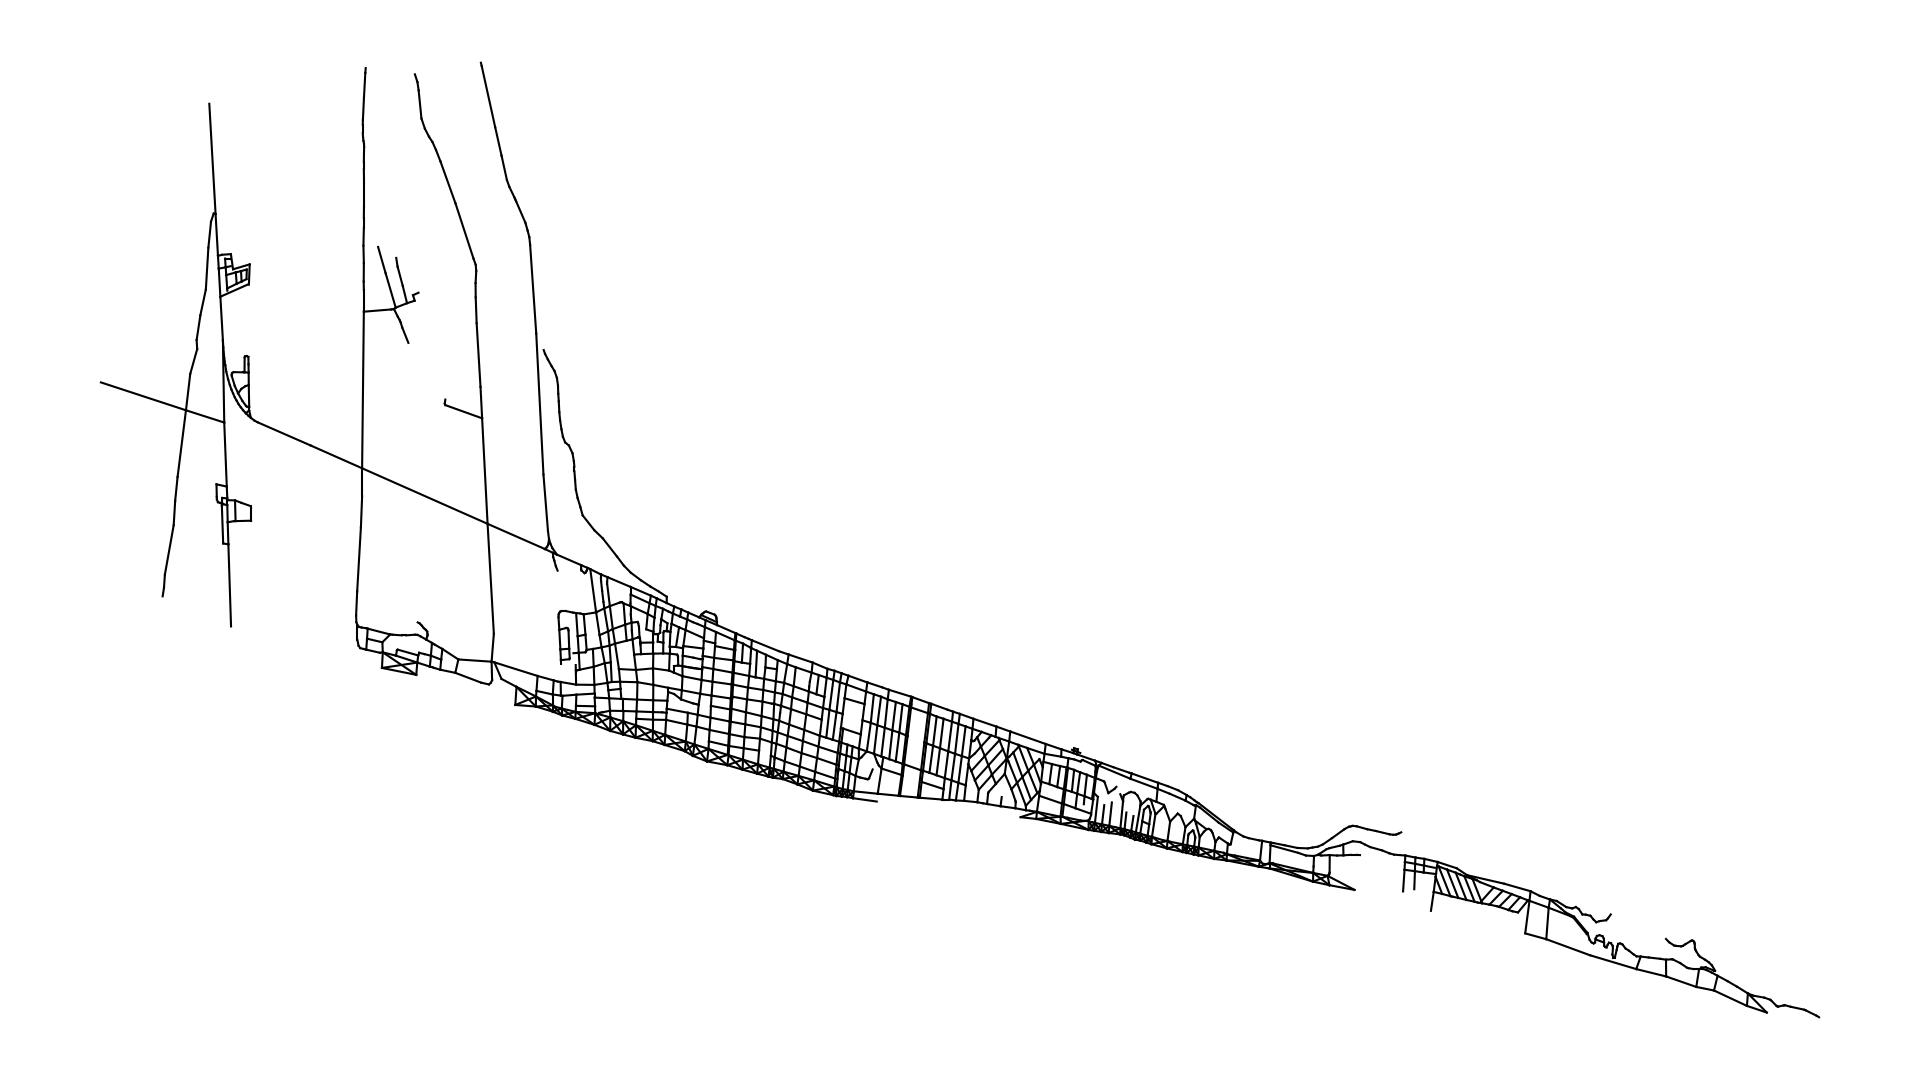
\includegraphics[width=0.85\textwidth]{figures/camana-city.png}
  \caption{Plan view of the city of the grid case.}
\end{figure}

\begin{itemize}
  \item \texttt{endTime}: Final evacuation time: 800 sec.
  \item \texttt{endNumberSimulation}: Final number of simulations: 7000.
  \item \texttt{meanRayleigh}: The mean value for the Rayleigh distribution. Average departure time
    of a person of 420 sec.
\end{itemize}

The \texttt{controlDict} file is shown below.
\begin{lstlisting}[style=control]
populationsFile  populationAtPoint.csv;

process calibration;

endTime         1800;

meanRayleigh   420;

endNumberSimulation 1000;
\end{lstlisting}

Finally, in the \texttt{postprocessing} folder there are files to perform visualizations of the data
externally to the main program. The file \texttt{snapshot.py} provides images at each time step. The
file \texttt{zoom.py} makes it possible to create images of a wide area to observe the evacuation
movement in detail, as shown in the following image.

\subsection{Python case}
If you want to use stateMatrix data from previous simulations, but from the Python version of the
same code, the \texttt{pythonVersion} command must be enabled. The \texttt{controlDict} of the grid
case using data exported from the Python code is shown below. This option must be enabled because
the order of the street connections at an intersection is different between the different
languages.

\end{document}
